\modeCorrection

\renewcommand{\thesubsection}{\textcolor{red}{\Roman{section}.\arabic{subsection}}}
\renewcommand{\thesubsubsection}{\textcolor{red}{\Roman{section}.\arabic{subsection}.\alph{subsubsection}}}

\setcounter{section}{0}
\sndEnTeteCoursQuatre

\begin{mdframed}[style=titr, leftmargin=60pt, rightmargin=60pt, innertopmargin=7pt, innerbottommargin=7pt, innerrightmargin=8pt, innerleftmargin=8pt]

\begin{center}
\large{\textbf{Chapitre 4 : Propagation de la lumière dans les milieux}}
\end{center}
\end{mdframed}
La lumière se propage-t'elle en ligne droite ? Quelles sont les lois qui gouvernent la propagation de la lumière ? Comment peut-on modéliser l'\oe il ?

\begin{tcolorbox}[colback=blue!5!white,colframe=blue!75!black,title=Mots clés du chapitre :]
Lois de Snell-Descartes, réfraction, réflexion, dispersion, lentille convergente.
\end{tcolorbox}


\section{Changement du milieu de propagation : lois de Snell-Descartes}
\subsection{Mise en évidence expérimentale}
\begin{wrapfigure}{r}{0.3\textwidth}
\vspace{-0cm}
    \centering
     
\includegraphics[width=0.32\textwidth]{Images/Cours/Chapitre_3/Haut_parleur_bougie.PNG}
   \end{wrapfigure}
\textcolor{green}{\underline{Expérience 1 :}} On place un laser face à un écran d'observation. On vaporise de l'eau sur le trajet de la lumière. Observations : \\
\textcolor{red}{En vaporisant de l'eau sur le parcours de la lumière, on observe que \underline{la lumière se propage en ligne droite}.}\\
\textcolor{green}{\underline{Expérience 2 :}} On place un laser face à un écran d'observation. On met sur le chemin de la lumière une bassine en verre transparent remplie d'eau. Observations : \\
\textbf{Observations :} \textcolor{red}{Par rapport à l'expérience 1, on remarque que la lumière du laser n'arrive pas au même endroit sur l'écran. Elle a été \underline{déviée}.}


\begin{tcolorbox}[colback=red!5!white,colframe=red!75!black,title=\textbf{Propriété de l'émission d'un son : }]
L'émission d'un signal sonore par un objet appelé \textcolor{red}{émetteur} résulte de la vibration de cet objet. Cette vibration se transmet fait vibrer les molécules dans l'air de proche en proche pour permettre sa \textcolor{red}{propagation}.
\end{tcolorbox}

\textcolor{blue}{Vidéo : les insectes les plus bruyants du monde !} \url{https://www.youtube.com/watch?v=qveMTTSAQPQ}
\begin{tcolorbox}[colback=red!5!white,colframe=red!75!black,title=\textbf{Caisse de résonance : }]
Une \textcolor{red}{caisse de résonance}permet de sélectionner et d'amplifier, c'est-à-dire augmenter son \textcolor{red}{amplitude} certains sons.
\end{tcolorbox}

\textbf{\underline{Exemple de caisse de résonance :}} Les instuments de musiques : flûte, guitare acoustique, contrebasse, etc.


\subsection{Approche expérimentale de la propagation}
\textcolor{green}{\underline{Expérience 2 :}} On place un réveil ou une alarme sur le plateau d'une cloche à vide. On met l'alarme en marche et on fait progressivement le vide (on retire l'air) sous la cloche. On mesure l'intensité du son au cours de l'expérience grâce à un sonomètre.
\begin{center}
    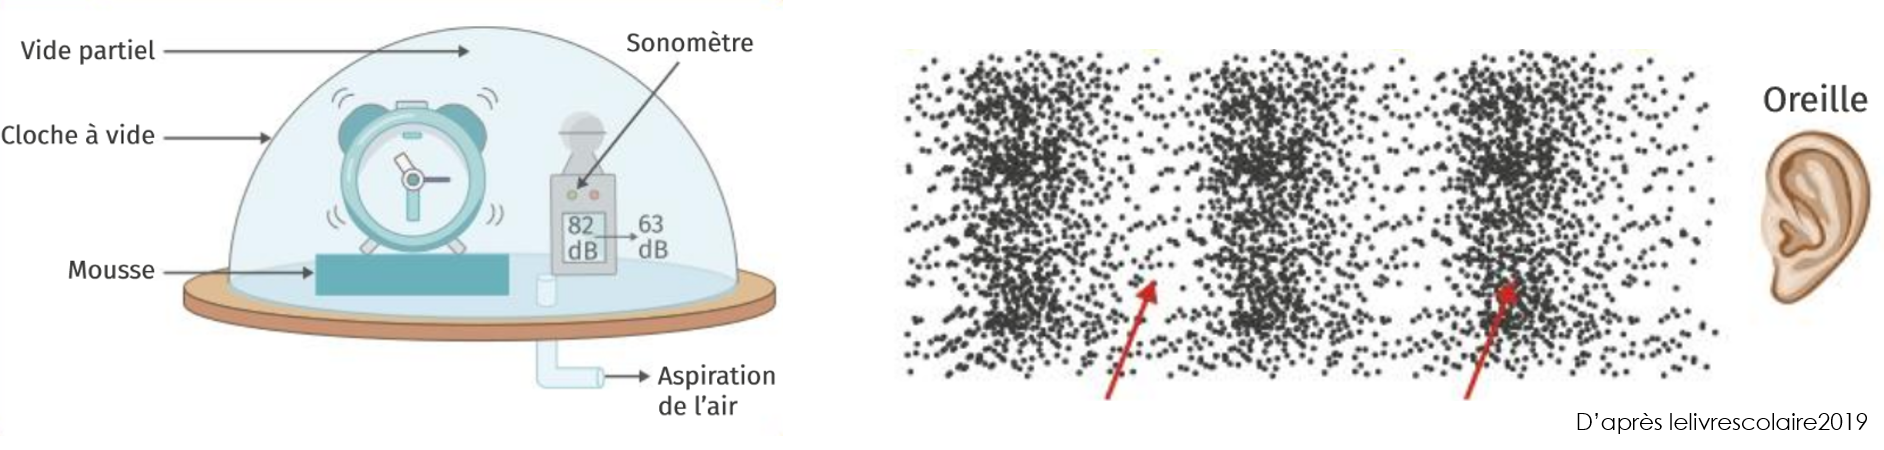
\includegraphics[scale=0.57]{Images/Cours/Chapitre_3/Propagation_exp.png}
\end{center}

\textbf{Observations :} On remarque que lorsqu'on retire progressivement l'air, le son de l'alarme semble atténué. Si la pompe a fonctionné suffisamment longtemps, on peut même ne plus entendre le son émis par l'alarme.

\begin{tcolorbox}[colback=red!5!white,colframe=red!75!black,title=\textbf{Propriété de la propagation du son : }]
Le son a besoin d'un \textcolor{red}{milieu matériel} pour se propager. Le signal se propage par suite de compressions et dilatations du milieu de propagation.
\end{tcolorbox}

Pour revoir l'expérience de la cloche à vide en vidéo : \url{https://www.youtube.com/watch?v=BC9Pod4cnpk}

\importantbox{Un signal sonore peut se propager dans un autre milieu matériel que l'air. Les baleines à bosses chantent sous l'eau pour communiquer entre elles et même choisir leur partenaire de reproduction sur des milliers de kilomètres !}

\section{Vitesse de propagation d'un signal sonore}
\begin{Large}
    \ding{43}
\end{Large}
Voir TP 7 : Mesure de la vitesse du son dans l'air.
\subsection{Définition}
\begin{tcolorbox}[colback=green!5!white,colframe=green!75!black,title=\textbf{Vitesse de propagation :}]
La \textcolor{red}{vitesse de propagation} $v$ d'un signal sonore est définie comme le rapport de la distance $d$ parcourue par ce signal sur le temps (ou durée) de propagation $\Delta t$ associé :
\begin{empheq}[box=\fbox]{equation*}
    v = \frac{d}{\Delta t}
\end{empheq}
$v$ s'exprime en m.s$^{-1}$, $d$ en m et $\Delta t$ en s.
\end{tcolorbox}
\subsection{Influence du milieu et de ses caractéristiques sur la vitesse de propagation du son}
\subsubsection{La température}
\`{A} partir du document 2 dans le TP 7 : \textit{Mesure de la vitesse des ondes sonores dans l'air}, compléter le tableau suivant :
\begin{center}
    \begin{tabular}{|C{0.4}|C{0.09}|C{0.09}|C{0.09}|C{0.09}|C{0.09}|}
\hline
     \cellcolor{blue!25}Température (en $\degreCelsius$) & -10 & 0 & 10 & 20 & 30 \\
     \hline 
     \cellcolor{blue!25}Vitesse de propagation du son dans l'air (en m.s$^{-1}$) & 325 & 332 & 337 & 343 & 349 \\
     \hline
\end{tabular}
\end{center}
\subsubsection{Le milieu de propagation}
\begin{center}
    \begin{tabular}{|C{0.4}|C{0.09}|C{0.09}|C{0.09}|C{0.09}|C{0.09}|}
\hline
     \cellcolor{blue!25}Milieu & air & eau & béton & acier \\
     \hline 
     \cellcolor{blue!25}Vitesse de propagation du son dans le milieu à 15$\degreCelsius$ (en m.s$^{-1}$) & 340 & 1480 & 3100 & 5600 \\
     \hline
\end{tabular}
\end{center}

\begin{tcolorbox}[colback=red!5!white,colframe=red!75!black,title=\textbf{Bilan sur la propagation du son dans un milieu : }]
La vitesse de propagation du son dépend du \textcolor{red}{milieu matériel de propagation} et des \textcolor{red}{caractéristiques physiques} de ce milieu (température, masse volumique, compressibilité) de celui-ci.\\

On retiendra qu'à T=15$\degreCelsius$ : 
\begin{empheq}[box=\fbox]{equation*}
    v_{son, air} \simeq 340~\text{m.s$^{-1}$}
\end{empheq}

\end{tcolorbox}


\subsection{Comparaison de $v_{son, air}$ avec d'autres valeurs de vitesses}
\begin{center}
    \begin{tabular}{|c|c|c|c|c|c|c|c|}
\hline
     \cellcolor{blue!25}Exemple & Escargot & Usain Bolt & Guépard & Son (à 15$\degreCelsius$)  & Ariane 5 & Lumière \\
     \hline 
     \cellcolor{blue!25}Vitesse (en m/s) & 0,001 & 10,44 & 36,1 & 340 & 10410 & 300 000 000\\
     \hline
\end{tabular}
\end{center}

%\begin{wrapfigure}{r}{0.3\textwidth}
%\vspace{-0.7cm}
%\centering
%     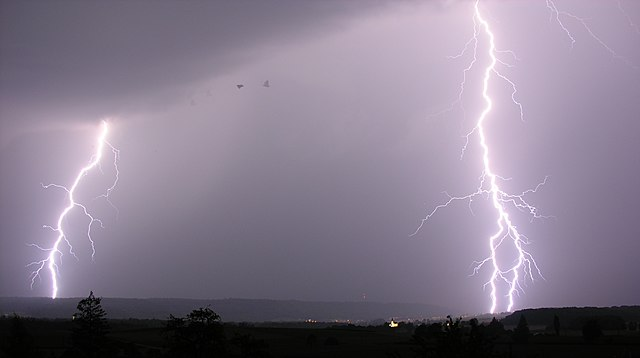
\includegraphics[width=0.3\textwidth]{Images/Cours/Chapitre_3/Eclair.JPG}
%   \end{wrapfigure}
\begin{mdframed}[style=autreexo]
\textbf{\bsc{Exercice de cours 1} - Distance d'un orage}\\
Un observateur observe un orage. L'air est lourd et affiche $30\degreCelsius$. Soudain, il voit le ciel s'éclairer et un éclair tomber. Il déclanche alors un chronomètre et mesure $\Delta t = 2,07$~s au moment où le grondement du tonnerre lui parvient. \`{A} quelle distance $d$ de l'observateur se situe l'éclair qui vient de tomber ?
\end{mdframed}
\textit{Réponse : D'après le cours et le tableau du cours, le son se propage à la vitesse $v_{son,30\degreCelsius}=\frac{d}{\Delta t}=349$~m.s$^{-1}$. On en déduit donc la distance entre l'observateur et l'orage :
\begin{equation*}
    d = v_{son,30\degreCelsius}\times \Delta t = 349\times 2,07 = 722~\text{m}
\end{equation*}}
\begin{Large}
    \ding{45}
\end{Large}\textbf{Exercice 5,7,9 et 10}

\section{Les signaux sonores périodiques}
%Nous nous intéressons dans cette section à décrire les caractéristiques d'un signal sonore : quels outils mathématiques peut-on utiliser pour décrire un son plus ou moins fort ? plus ou moins aigu ? Comment peut-on visualiser un signal sonore en physique ?
\subsection{\og Voir \fg ~un son à l'aide d'une chaîne de mesure}
\begin{tcolorbox}[colback=green!5!white,colframe=green!75!black,title=\textbf{Microphone et enregistrement:}]
Un microphone est un capteur qui convertit un signal sonore reçu en une tension électrique $U$ en volt. Le signal électrique produit par le microphone est ensuite enregistré sur une carte de mesure relié à un ordinateur qui permet d'afficher et anayser le signal sonore.
\begin{center}
    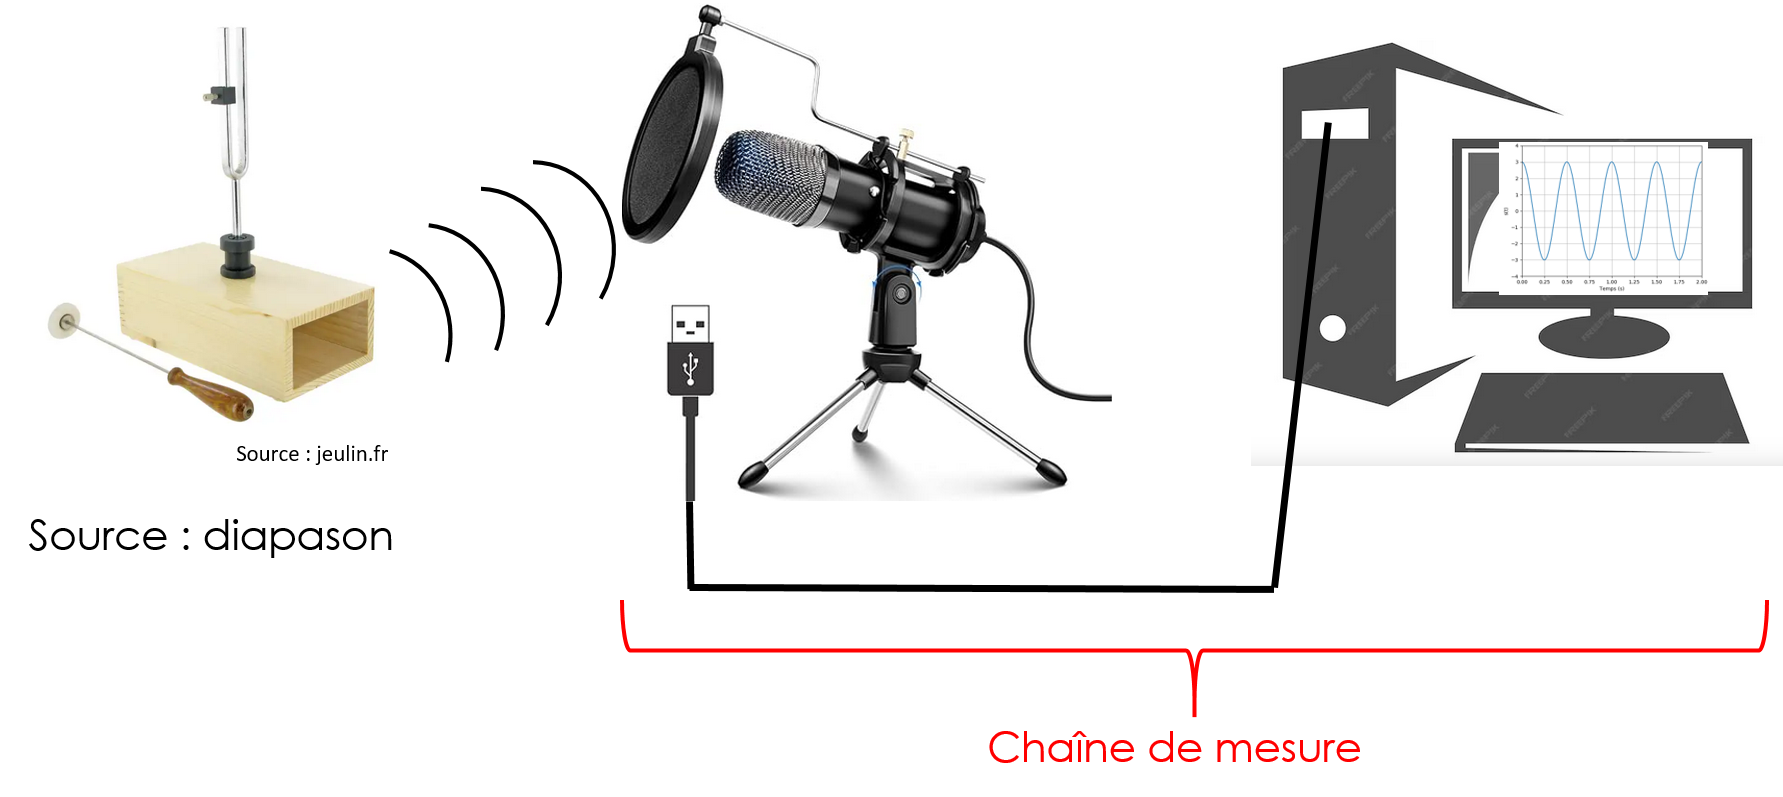
\includegraphics[scale = 0.5]{Images/Cours/Chapitre_3/Chaine_mesure.png}
\end{center}
\end{tcolorbox}
\subsection{Définition d'un signal sonore périodique}
\textcolor{green}{Expérience 3 :} On joue une note à l'aide d'un diapason (voir la figure ci-dessus), le signal est amplifié par une caisse de résonance devant laquelle est placé un microphone. Le signal produit est le suivant :
\begin{multicols}{2}
\begin{center}
    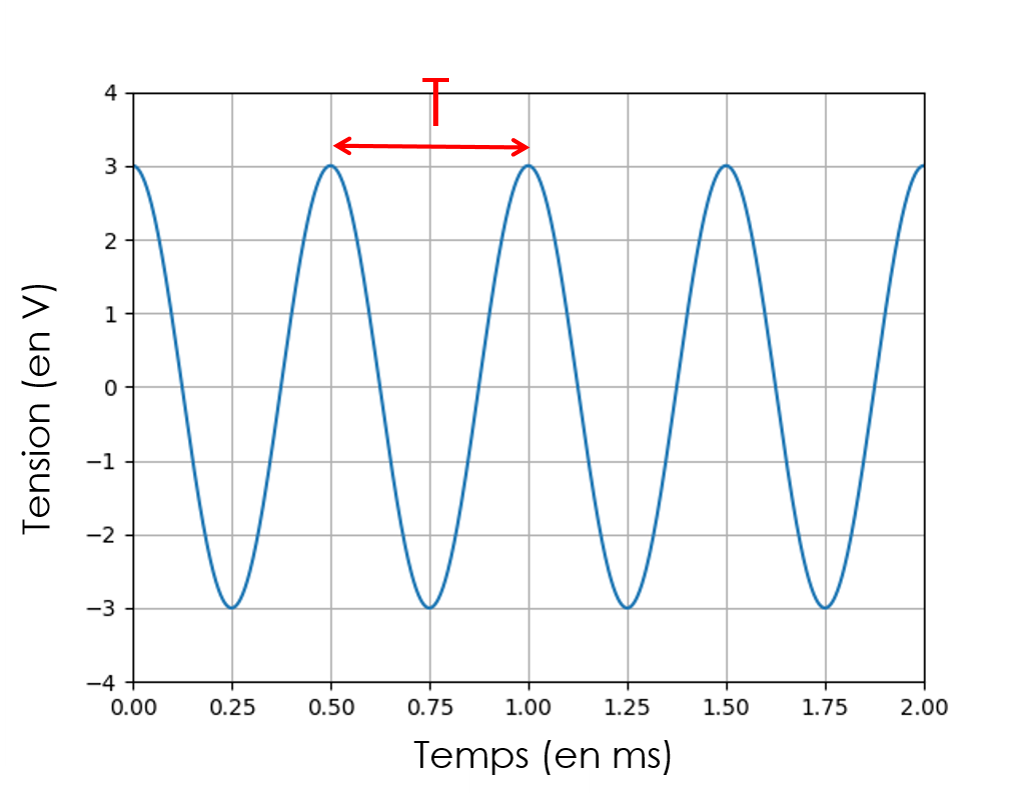
\includegraphics[scale=0.4]{Images/Cours/Chapitre_3/Signal_diapason_freq.png}
\end{center}
\begin{tcolorbox}
[colback=green!5!white,colframe=green!75!black,title=\textbf{Signal périodique :}]
Un signal sonore \textcolor{red}{périodique} est un signal qui se \textcolor{red}{reproduit à l'identique} au cours du temps.
\begin{center}
    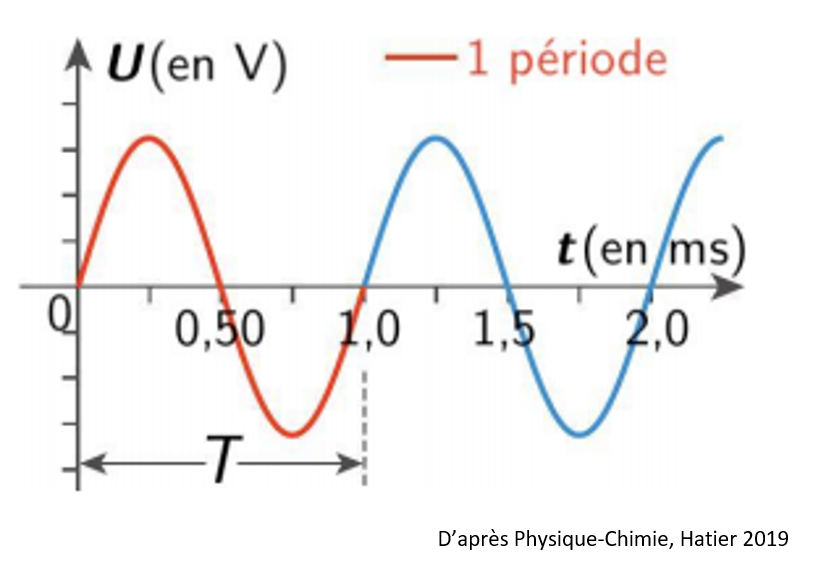
\includegraphics[scale=0.35]{Images/Cours/Chapitre_3/Periode.PNG}
\end{center}
\end{tcolorbox}
\end{multicols}

\subsection{Période et fréquence}
\begin{tcolorbox}
[colback=green!5!white,colframe=green!75!black,title=\textbf{Période :}]
La période est la plus petite durée au bout de laquelle le signal se reproduit identiquement à lui-même. Elle se note $T$ et s'exprime en secondes (s). 
\end{tcolorbox}
\begin{mdframed}[style=autreexo]
\textbf{\bsc{Exercice de cours 2} - Période du son émis par un diapason}\\
\question{Représenter sur le graphique ci-dessus la période $T$ du signal sonore émis par le diapason. Que vaut cette période ?}{Voir le graphique. On mesure $T=0.5$~ms.}{0}
\\
\question{Comment améliorer la précision de la mesure ?}{On peut mesurer plusieurs périodes pour augmenter la précision de la mesure. L'incertitude obtenue par la mesure d'une période sera alors divisée par le nombre de périodes mesurées.}{0}
\end{mdframed}

\begin{tcolorbox}
[colback=green!5!white,colframe=green!75!black,title=\textbf{Fréquence :}]
La fréquence $f$ d'un signal sonore périodique est le nombre de répétitions de ce signal par unité de temps. C'est l'inverse de la période $T$ :
\begin{empheq}[box=\fbox]{equation*}
    f = \frac{1}{T}
\end{empheq}
Elle s'exprime en Hertz (Hz) où s$^{-1}$.
\end{tcolorbox}

%%%%%%%%
%\newpage
%%%%%%%%

\begin{mdframed}[style=autreexo]
\textbf{\bsc{Exercice de cours 3} - Fréquence sonore du diapason}\\
\question{Calculer la fréquence du signal sonore du diapason}{On sait que $T=0.5$~ms. On en déduit $f=\frac{1}{T}=\frac{1}{0,5\times 10^{-3}}=2000$~Hz.}{0}
\end{mdframed}
\begin{Large}
    \ding{45}
\end{Large}\textbf{Exercice 8 et 13}

%%%%%%%%
\newpage
%%%%%%%%

\subsection{Hauteur et timbre d'un son}
\begin{Large}
    \ding{43}
\end{Large} Voir \textit{TP 8 : Mieux connaître sa voix}
\begin{multicols}{2}
    \begin{tcolorbox}[colback=green!5!white,colframe=green!75!black,title=\textbf{Hauteur :}]
        La \textcolor{red}{hauteur} d'un son est une caractéristique reliée à la fréquence de ce son. Elle permet de distinguer un son grave d'un son aigu : un son aigu a une fréquence plus grande qu'un son grave.
    \end{tcolorbox}
    \begin{tcolorbox}[colback=green!5!white,colframe=green!75!black,title=\textbf{Timbre :}]
        Le \textcolor{red}{timbre} d'un son ou d'un instrument de musique est lié à sa \textcolor{red}{perception} par l'oreille. Deux sons de même hauteur, joués par deux instruments de musique différents ont des timbres différens comme on peut le voir sur la figure de droite.
    \end{tcolorbox}
    
    \begin{center}
        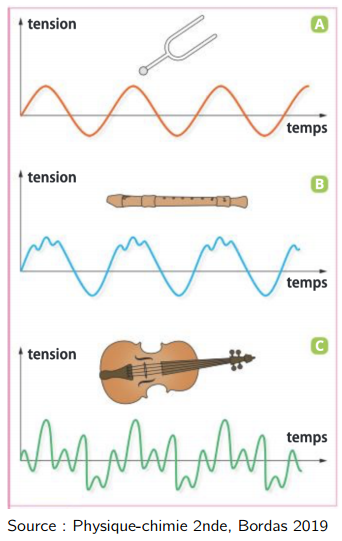
\includegraphics[scale=1.1]{Images/Cours/Chapitre_3/Timbres_2.PNG}
    \end{center}
\end{multicols}

\section{Perception d'un son par l'oreille}
\subsection{Domaines de fréquence des signaux sonores}
\begin{tcolorbox}[colback=red!5!white,colframe=red!75!black,title=\textbf{Fréquences des signaux sonores : }]
Un son est un signal sonore audible pour l'être humain dont la fréquence est comprise entre 20 et 20 000 Hz.
\begin{center}
    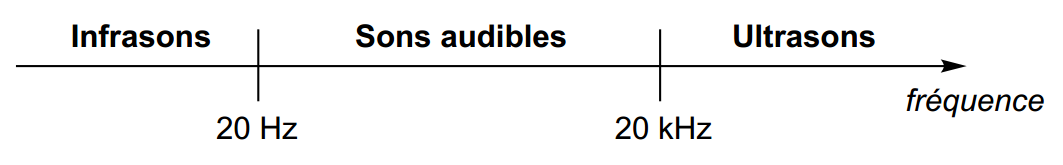
\includegraphics[scale=0.7]{Images/Cours/Chapitre_3/domaine_freq.PNG}
\end{center}
Les \textcolor{red}{infrasons} et les \textcolor{red}{ultrasons} sont des signaux inaudibles pour l'être humain.
\end{tcolorbox}
\begin{Large}
    \ding{45}
\end{Large}\textbf{Exercice 12 et 25}



\subsection{Intensité sonore et niveau d'intensité sonore}
\begin{tcolorbox}[colback=green!5!white,colframe=green!75!black,title=\textbf{Définition :}]
\begin{multicols}{2}
\begin{itemize}[label=\textbullet]
    \item L'\textcolor{red}{intensité sonore}, qu'on note I, est une grandeur liée à l'\textcolor{red}{amplitude} du signal sonore. L'intensité s'exprime en watts par mètre carré (W.m$^{-2}$). Plus l'amplitude du son est grande, plus l'intensité sonore est grande.
    \item Le niveau d'intensité sonore, noté $L$, est une grandeur liée à l'intensité sonore et traduit la perception du son par l'oreille humaine. Il s'exprime en décibel (dB). Le niveau d'intensité sonore se mesure avec un \textcolor{red}{sonomètre}.
    \end{itemize}

\begin{center}
    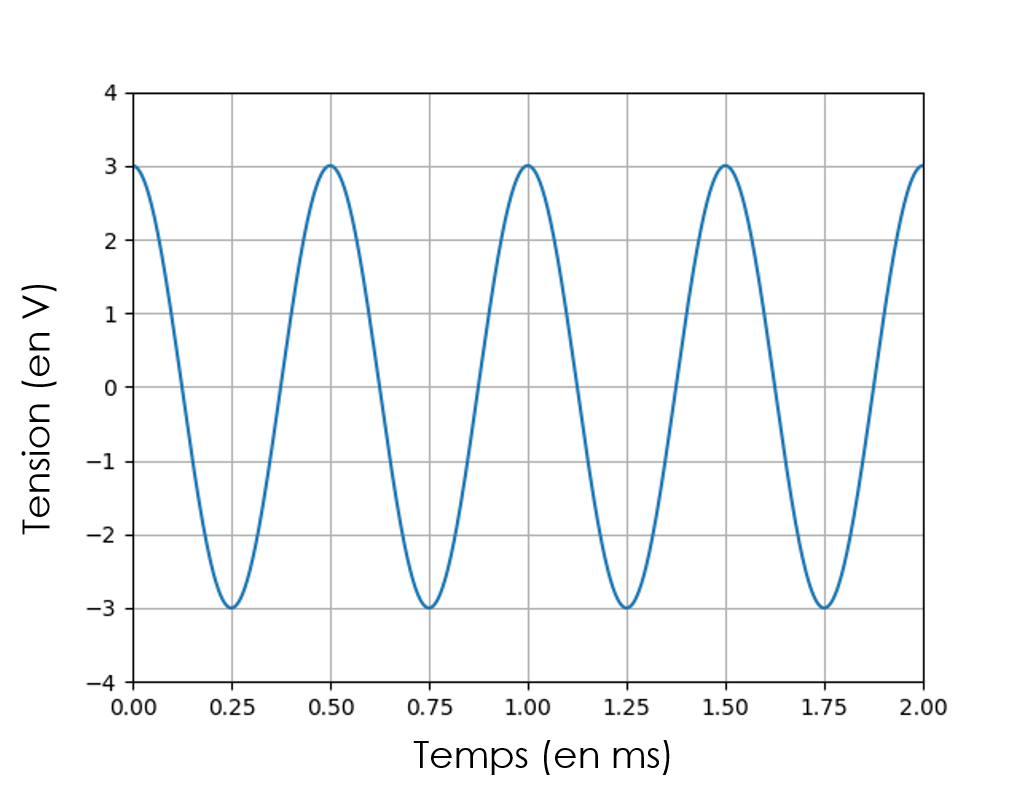
\includegraphics[width=0.35\textwidth]{Images/Cours/Chapitre_3/Signal_diapason.PNG}
\end{center}
\begin{center}
    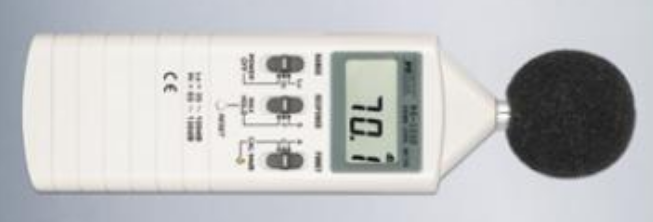
\includegraphics[width=0.35\textwidth]{Images/Cours/Chapitre_3/Sonometre.PNG}
\end{center}
\end{multicols}
\end{tcolorbox}

\importantbox{L'intensité sonore et le niveau sonore ne sont pas proportionnels : si l'intensité sonore est doublée, le niveau d'intensité sonore n'augmente \og que \fg~de 3dB. L'oreille ne perçoit donc pas un son deux fois plus fort mais \og un peu \fg~plus fort.}
\begin{center}
    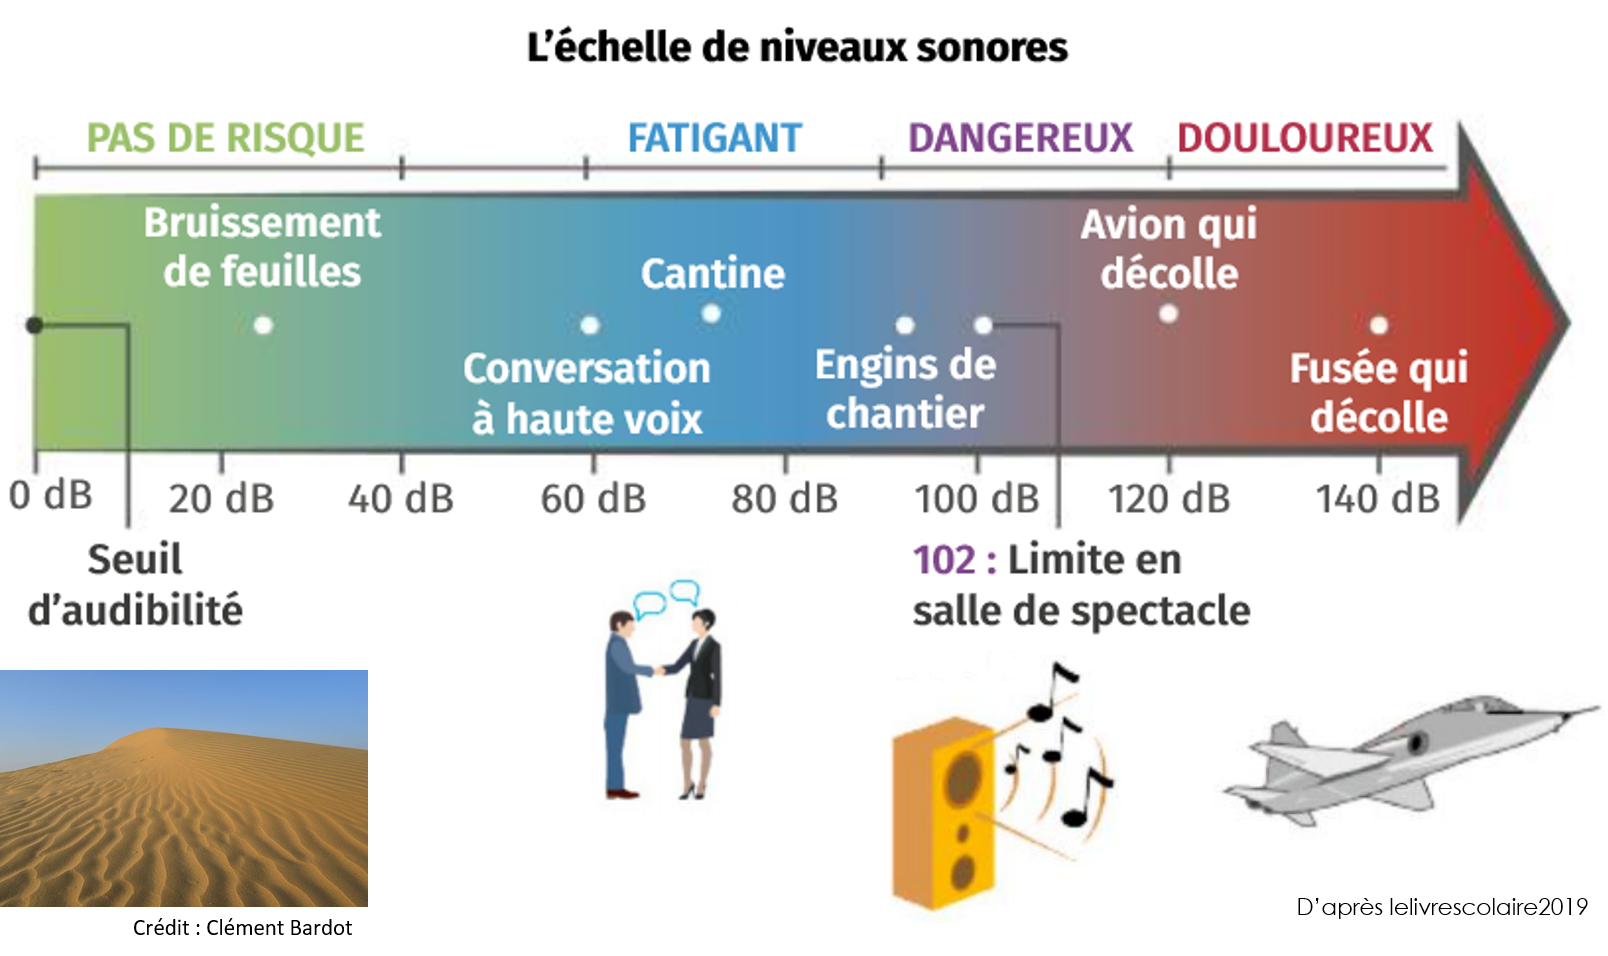
\includegraphics[scale=0.65]{Images/Cours/Chapitre_3/Echelle_niveau_sonore.PNG}
\end{center}
\begin{Large}
    \ding{45}
\end{Large}\textbf{Exercice 22 et 27}